\section{Theorie}
\label{sec:Theorie}

% In knapper Form sind die physikalischen Grundlagen des Versuches, des Messverfahrens, sowie sämtliche für die Auswertung erforderlichen Gleichungen darzustellen. (Keine Herleitung)

% (eventuell die Aufgaben)

% Der Versuchsaufbau: Beschreibung des Versuchs und der Funktionsweise (mit Skizze/Bild/Foto)

% Formeln zum Abarbeiten
% -Ladungsträger pro Volumen n
% -Ladungsträger pro Atom z
% -mittlere Flugzeit
% -Driftgeschw.
% -Beweglichkeit
% -Totalgeschw.
% -mittlere freie Weglänge
% -

%%%%%%%%%%

Ein Material wird elektrisch leitend genannt, wenn durch dieses elektrische Ladungen fließen können.
Dabei wird in den meisten Fällen davon ausgegangen, dass der Strom aus negativen Ladungen, also Elektronen besteht.

Da die meisten Metalle freie Elektronen, auch Leitungselektronen genannt, aufweisen, sind diese besonders leitfähig und werden hier näher untersucht.

Die Energieniveaus von Metallatomen sind diskret und können in verschiedene Energiebänder aufgeteilt werden. 
Dabei sind z.B. beim Alkali-Metall die 1s, 2s und 2p Bänder des Na Atoms immer voll mit Elektronen besetzt und diese können weder Energie aufnehmen noch abgeben.
Das 3s Band ist allerdings nur mit einem Elektron gefüllt. 
Daher können Elektronen in diesem Band Energie aufnehmen und bewegen sich bei angelegtem Elektrischen Feld entlang dessen Feldlinien.
So entsteht die elektrische Leitfähigkeit von Metallen. \cite{V311}

Allerdings bedeutet dies nicht, dass ein Metall perfekt leitend ist und die Elektronen ungehindert fließen können.
Die Elektronen stoßen ständig mit anderen Teilchen zusammen und werden so verlangsamt.
Die gemittelte Zeit zwischen diesen Zusammenstößen heißt mittlere Flugzeit $\bar{\tau}$ und die gemittelte zurückgelegte Distanz heißt mittlere freie Weglänge $\bar{l}$.

Wie gut ein Stück Metall leitet beschreibt der sogenannte elektrische Widerstand.
Dieser ist über 
\begin{equation}
    R = 2\frac{m_0}{e_0}\frac{1}{n \cdot \bar{\tau}}\frac{L}{Q}
    \label{eq:widerstand}
\end{equation}
definiert.
Das geometrieunabhängige Äquivalent dazu ist der spezifische Widerstand
\begin{equation}
    \rho = R\frac{Q}{L}.
    \label{eq:spezwiderstand}
\end{equation}
Hier ist $m_0$ die Ruhemasse eines Elektrons, $e_0$ dessen Ladung, $n$ die Ladungsträgerdichte, $L$ die Länge des Leiters und $Q$ die Querschnittsfläche des Leiters. \cite{V311}

Somit kann die mittlere Flugzeit über 
\begin{equation}
    \bar{\tau} = 2\frac{m_0}{e_0}\frac{1}{n \cdot R}\frac{L}{Q} = 2\frac{m_0}{e_0}\frac{1}{n \cdot \rho}
    \label{eq:tau}
\end{equation}
berechnet werden. \cite{V311}

Bei einem angelegten äußeren elektrischen Feld $E$ besitzen die Elektronen eine mittlere Driftgeschwindigkeit $\bar{v}_\text{d}$ in dessen Richtung welche über 
\begin{equation}
    \bar{v}_\text{d} = -\frac{j}{n \cdot e_0}
    \label{eq:driftgeschwindigkeit}
\end{equation}
berechnet werden kann, wenn die Stromdichte $j$ bekannt ist. \cite{V311}

Zwischen der Driftgeschwindigkeit und der elektrischen Feldstärke besteht der Zusammenhang
\begin{equation}
    \bar{v}_\text{d} = \mu \cdot E
\end{equation}
wobei $\mu$ als Beweglichkeit bezeichnet wird. \cite{V311}

Mit 
\begin{equation}
    E = 2 \frac{m_0}{e_0^2}\frac{j}{n\cdot\bar{\tau}}
\end{equation}
kann die Beweglichkeit also über
\begin{equation}
    \mu = \frac{1}{2}\frac{e_0^2}{m_0}\frac{n\cdot\bar{\tau}}{j} \bar{v_\text{d}}
    \label{eq:beweglichkeit}
\end{equation}
berechnet werden.

Wenn die Bewegung der Elektronen durch Wärme zusätzlich beachtet wird, kann deren mittlere Totalgeschwindigkeit über
\begin{equation}
    \bar{v}_\text{total} = \sqrt{\frac{2 E_\text{F}}{m_0}}
    \label{eq:totalgeschwindigkeit}
\end{equation}
bestimmt werden wobei $E_\text{F}$ die sogenannte Fermi-Energie ist.
Diese kann über 
\begin{equation}
    E_\text{F} = \frac{\hbar^2}{2 m_0}\sqrt[3]{\left(\frac{3n}{8\symup{\pi}}\right)^2}
    \label{eq:fermienergie}
\end{equation}
mit dem Plankschen Wirkungsquantum $\hbar$ bestimmt werden. \cite{V311}

Somit kann die mittlere freie Weglänge über
\begin{equation}
    \bar{l} = \bar{\tau} \cdot \bar{v}_\text{total}
    \label{eq:weglaenge}
\end{equation}
berechnet werden.

In diesem Versuch werden alle Größen über den Hall-Effekt untersucht.
\begin{figure}
    \centering
    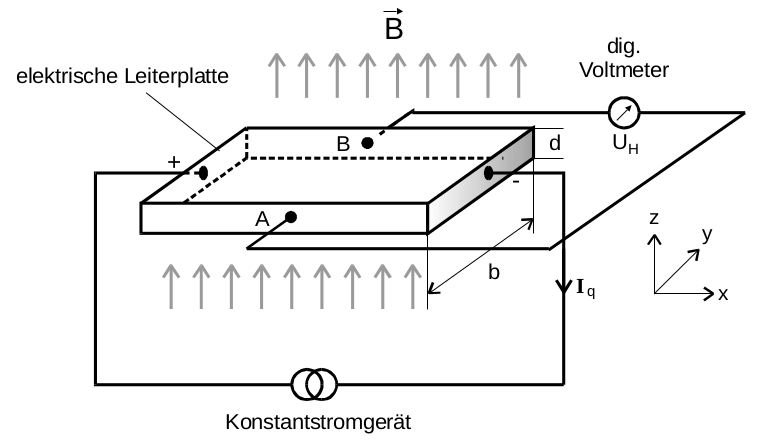
\includegraphics[width=0.5\textwidth]{images/skizze_1.png}
    \caption{Schematischer Versuchsaufbau zur Untersuchung des Hall-Effektes\cite{V311}}
    \label{fig:skizze_1}
\end{figure}
Wenn wie in \autoref{fig:skizze_1} gezeigt ein Strom durch eine Platte fließt und senkrecht dazu ein Magnetfeld angelegt wird, entsteht eine Spannung zwischen den Punkten A und B.
Diese Spannung wird durch die Lorentz-Kraft verursacht und kann über
\begin{equation}
    U_\text{H} = -\frac{B \cdot I_\text{q}}{n \cdot e_0 \cdot d}
    \label{eq:hallspannung}
\end{equation}
berechnet werden. 
Hier ist $d$ die Dicke der Platte, $B$ die Magnetfeldstärke und $I_\text{q}$ die Stromstärke des Querstroms.
Diese Spannung wird Hall-Spannung genannt und das Phänomen wird Hall-Effekt genannt.\cite{V311}

